\documentclass[10pt,a4paper]{article}
\usepackage[utf8]{inputenc}
\usepackage{amsmath}
\usepackage{amsfonts}
\usepackage{amssymb}
\usepackage[hidelinks]{hyperref}
\usepackage{cleveref}
\usepackage{tikz}
\usepackage{listings}
\usepackage{float}
\usepackage{fullpage}
\author{Daniel Underwood}
\title{Linear System Solution of Poisson Equation on Dirichlet Boundary}

\newcommand{\crefrangeconjunction}{--}

\usepackage{color} %red, green, blue, yellow, cyan, magenta, black, white
\definecolor{mygreen}{RGB}{28,172,0} % color values Red, Green, Blue
\definecolor{mylilas}{RGB}{170,55,241}


\begin{document}
\maketitle

\lstset{language=Matlab,%
    %basicstyle=\color{red},
    breaklines=true,%
    morekeywords={matlab2tikz},
    keywordstyle=\color{blue},%
    morekeywords=[2]{1}, keywordstyle=[2]{\color{black}},
    identifierstyle=\color{black},%
    stringstyle=\color{mylilas},
    commentstyle=\color{mygreen},%
    showstringspaces=false,%without this there will be a symbol in the places where there is a space
    numbers=left,%
    numberstyle={\small \color{gray}},% size of the numbers
    numbersep=9pt, % this defines how far the numbers are from the text
    emph=[1]{for,end,break},emphstyle=[1]\color{red}, %some words to emphasise
    %emph=[2]{word1,word2}, emphstyle=[2]{style},    
}


\section*{Introduction}
The Dirichlet boundary value problem is a boundary value problem in which the function on the boundary is defined by a function; that is

\begin{subequations}
  \begin{align}
  \hat{\mathcal{D}} u(x_1 , ... , x_n) &= f(x_1 , ... , x_n) \label{eqn: dirichlet 1}\\
  u(x_1, ..., x_n) &= g(x_1, ..., x_n) \,\, \text{for} \,\, (x_1, ..., x_n) \in \partial\Omega \label{eqn: dirichlet 2}
  \end{align}
\end{subequations}

where $\hat{\mathcal{D}}$ is a linear differential operator consisting of a sum of derivatives of any order including mixed derivatives and $u$, $f$, and $g$ are functions of $n$ variables from $\mathbb{R}^n$ to $\mathbb{R}$. The problem is solved on a domain $\Omega \subset \mathbb{R}^n$ with a boundary $\partial \Omega$. In simpler terms, a Dirichlet problem is a boundary value problem in which the solution value is given in terms of a function, rather than other conditions such as the value of the solution's derivative on the boundary that is given in a Neumann problem.

The Dirichlet problem is very useful in a variety of fields. Differential equations frequently used with Dirichlet boundary conditions include the  Laplace equation, Poisson equation, heat/diffusion, and wave equation. These equations are seen quite often and the latter three are actually all more general forms of the Laplace equation; the Poisson equation is a non-homogeneous form while the heat/diffusion and wave equations add first and second time derivative terms, respectively.

The Laplace equation

\begin{equation}
\Delta u = 0 \label{eqn: laplace}
\end{equation}

is one of the most basic partial differential equations used with Dirichlet boundary conditions. The solutions to this equations are harmonic functions. The Laplace equation has uses in various fields of physics to describe potentials due to forces such as gravity, the electromagnetic force, and fluid forces. It it also the steady-state heat or diffusion equation as well as the steady-state wave equation by taking $u_t = 0$ in \cref{eqn: diffusion} or $u_{tt} = 0$ in the $\Box$ operator of \cref{eqn: wave}. The solutions of the Laplace equation are harmonic functions.

The Poisson equation

\begin{equation}
\Delta u = f \label{eqn: poisson}
\end{equation}

Is the non-homogeneous form of \cref{eqn: laplace}. The Poisson equation has uses throughout physics as $f$ can be used to represent forces such as gravity, electromagnetism, and fluid forces. In these cases, $u$ represents a potential, which can be related to a force via Newton's second law or can be used in energy analysis. The $f$ term comes from a source. In the case of an electrostatic field, we have $f = - \frac{\rho (r)}{\epsilon_0}$, where $\rho$ is the radial charge density; the gravitational source term is $f = 4 \pi^2 G \rho(r)$, where $G$ is the universal gravitational constant and $\rho$ is the radial mass density.

The heat or diffusion equation

\begin{equation}
u_t - a \Delta u = 0 \label{eqn: diffusion}
\end{equation}

is a frequently used partial differential equation to represent the transfer of heat on the domain of a piece of material or the diffusion of a fluid through another fluid. $a$ is either the heat transfer coefficient or the diffusion coefficient depending on the usage case. It is frequently constant as a simplification, but can vary with position or time in more complicated cases. In these cases, the divergence term affects the transfer function and the equation will take on a slightly different form.

The wave equation

\begin{equation}
\Box u = 0 \label{eqn: wave}
\end{equation}

where $\Box \equiv \frac{1}{c^2} \frac{\partial^2}{\partial t^2} - \Delta$ is the d'Alembert operator with $c$ being the wave speed. The wave equation has usage throughout physics. In classical mechanics, the wave equation is used to represent oscillations and is the start to the large field of wave mechanics. Electromagnetism and quantum mechanics have their own wave equations, being Maxwell's equations for electromagnetism and the Schr{\"o}dinger equation in quantum mechanics.

\section*{Mathematical Theory}
There are many ways to solve \crefrange{eqn: laplace}{eqn: wave}. Analytically, they may be solved by separation of variables for many cases and in the case of Dirichlet boundary conditions may be solved by using Green's function; however, both of these techniques can become very difficult or even impossible depending on the domain on which the problem is being solved. Due to this difficulty, numerical methods start becoming highly favorable. While numerical methods do not yield a solution in terms of analytic functions, they can give a good idea of the behavior of the solution and parameters can be adjusted to make the error within an acceptable range. Additionally, once written, numerical methods can be used on a variety of variations of the problem and are often solved much quicker than a human could solve the same equation if a solution exists. Numerical data can even be fitted by functions to make guesses of analytic solutions or approximations.

Numerical solutions represent discrete relations rather than continuous ones and can be formulated by transforming the differential equation into a linear system. In this case, we have Poisson's equation with a Dirichlet boundary on a domain $\Omega \subset \mathbb{R}^2$

\begin{subequations}
  \begin{align}
  -u_{xx} - u_{yy} &= f(x, y) & \\
  u(x, y) &= 0 \,\, \text{for} \,\, (x, y) \in \partial \Omega
  \end{align}
\end{subequations}

The domain $\Omega$ is shown in \cref{fig: domain}. The domain could be scaled to arbitrary sizes, so it is easiest to take the squares making up $\Omega$ to be unit squares.

\begin{figure}[H]
\center
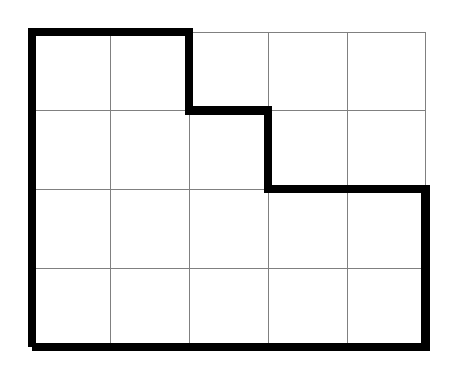
\begin{tikzpicture}
\draw[help lines] (0,0) grid (5,4);
\draw[line width=3] (0,0) -- (5,0) -- (5,2) -- (3,2) -- (3,3) -- (2,3) -- (2,4) -- (0,4) -- (0,0);
\end{tikzpicture}
\caption{Domain $\Omega$}
\label{fig: domain}
\end{figure}

To solve a differential equation numerically, we must discretize the differential operator into steps. A starting point for this is the limit definition of a derivative

\begin{equation}
\label{eqn: limit derivative}
f'(a) = \lim\limits_{h \to 0} \frac{f(a + h) - f(a)}{h}
\end{equation}

To discretize this limit, we take $h \to \Delta h$, where $\Delta h$ is small and taken to be smaller to achieve more accurate results. This relation can be used with a Taylor series to find relations for higher-order derivatives. Applying this to find the Laplace operator for $\mathbb{R}^2$ and indexing values yields the algebraic relation

\begin{equation}
\label{eqn: laplacian algebra}
- \Delta u(x_i, y_j) = \frac{4u_{ij} - u_{i+1, j} - u_{i+1, j} - u_{i, j+1} - u_{i, j-1}}{\left( \Delta h \right)^2}
\end{equation}

With \cref{eqn: laplacian algebra}, an operator matrix $\hat{A}$ may be formed such that $\hat{A} \vec{u}$ is a discretized form of $\Delta u$ for $\vec{u}$ is a vector formed by $u(x_i, y_j)$, where $x_i$ and $y_j$ are  points that are created when the boundary $\Omega$ is separated into a mesh with step size $\Delta h$. We then obtain a linear system

\begin{equation}
\label{eqn: linear system}
\hat{A} \vec{u} = \vec{f}
\end{equation}

where $\vec{f}$ is the vector created from $f(x_i, y_j)$ evaluated at the same mesh points as $\vec{u}$. 

This system can be solved by several different methods. To simplify the computation, the $\Delta h$ term is factored out of $\hat{A}$ and placed with the function term

\begin{equation}
\label{eqn: linear system 2}
\tilde{\hat{A}} \vec{u}  = \left( \Delta h \right)^2 \vec{f}
\end{equation}

 where $\tilde{\hat{A}} \equiv \left( \Delta h \right)^{-2} \hat{A}$. With this system defined by the operator in \cref{eqn: laplacian algebra}, we have an error of order $\left( \Delta h \right)^4$.

 \section*{Large Step Sizes}

 
 The system in \cref{eqn: linear system 2} can be explicitly solved relatively easily for small step sizes. This was done for step sizes of $h=1$ and $h = \frac{1}{2}$ in listings \ref{lst: explicit1}--\ref{lst: explicit12}, respectively. In these cases, the operator matrices were manually assigned with values of $-1$ for interacting points.

 \begin{figure}[H]
	 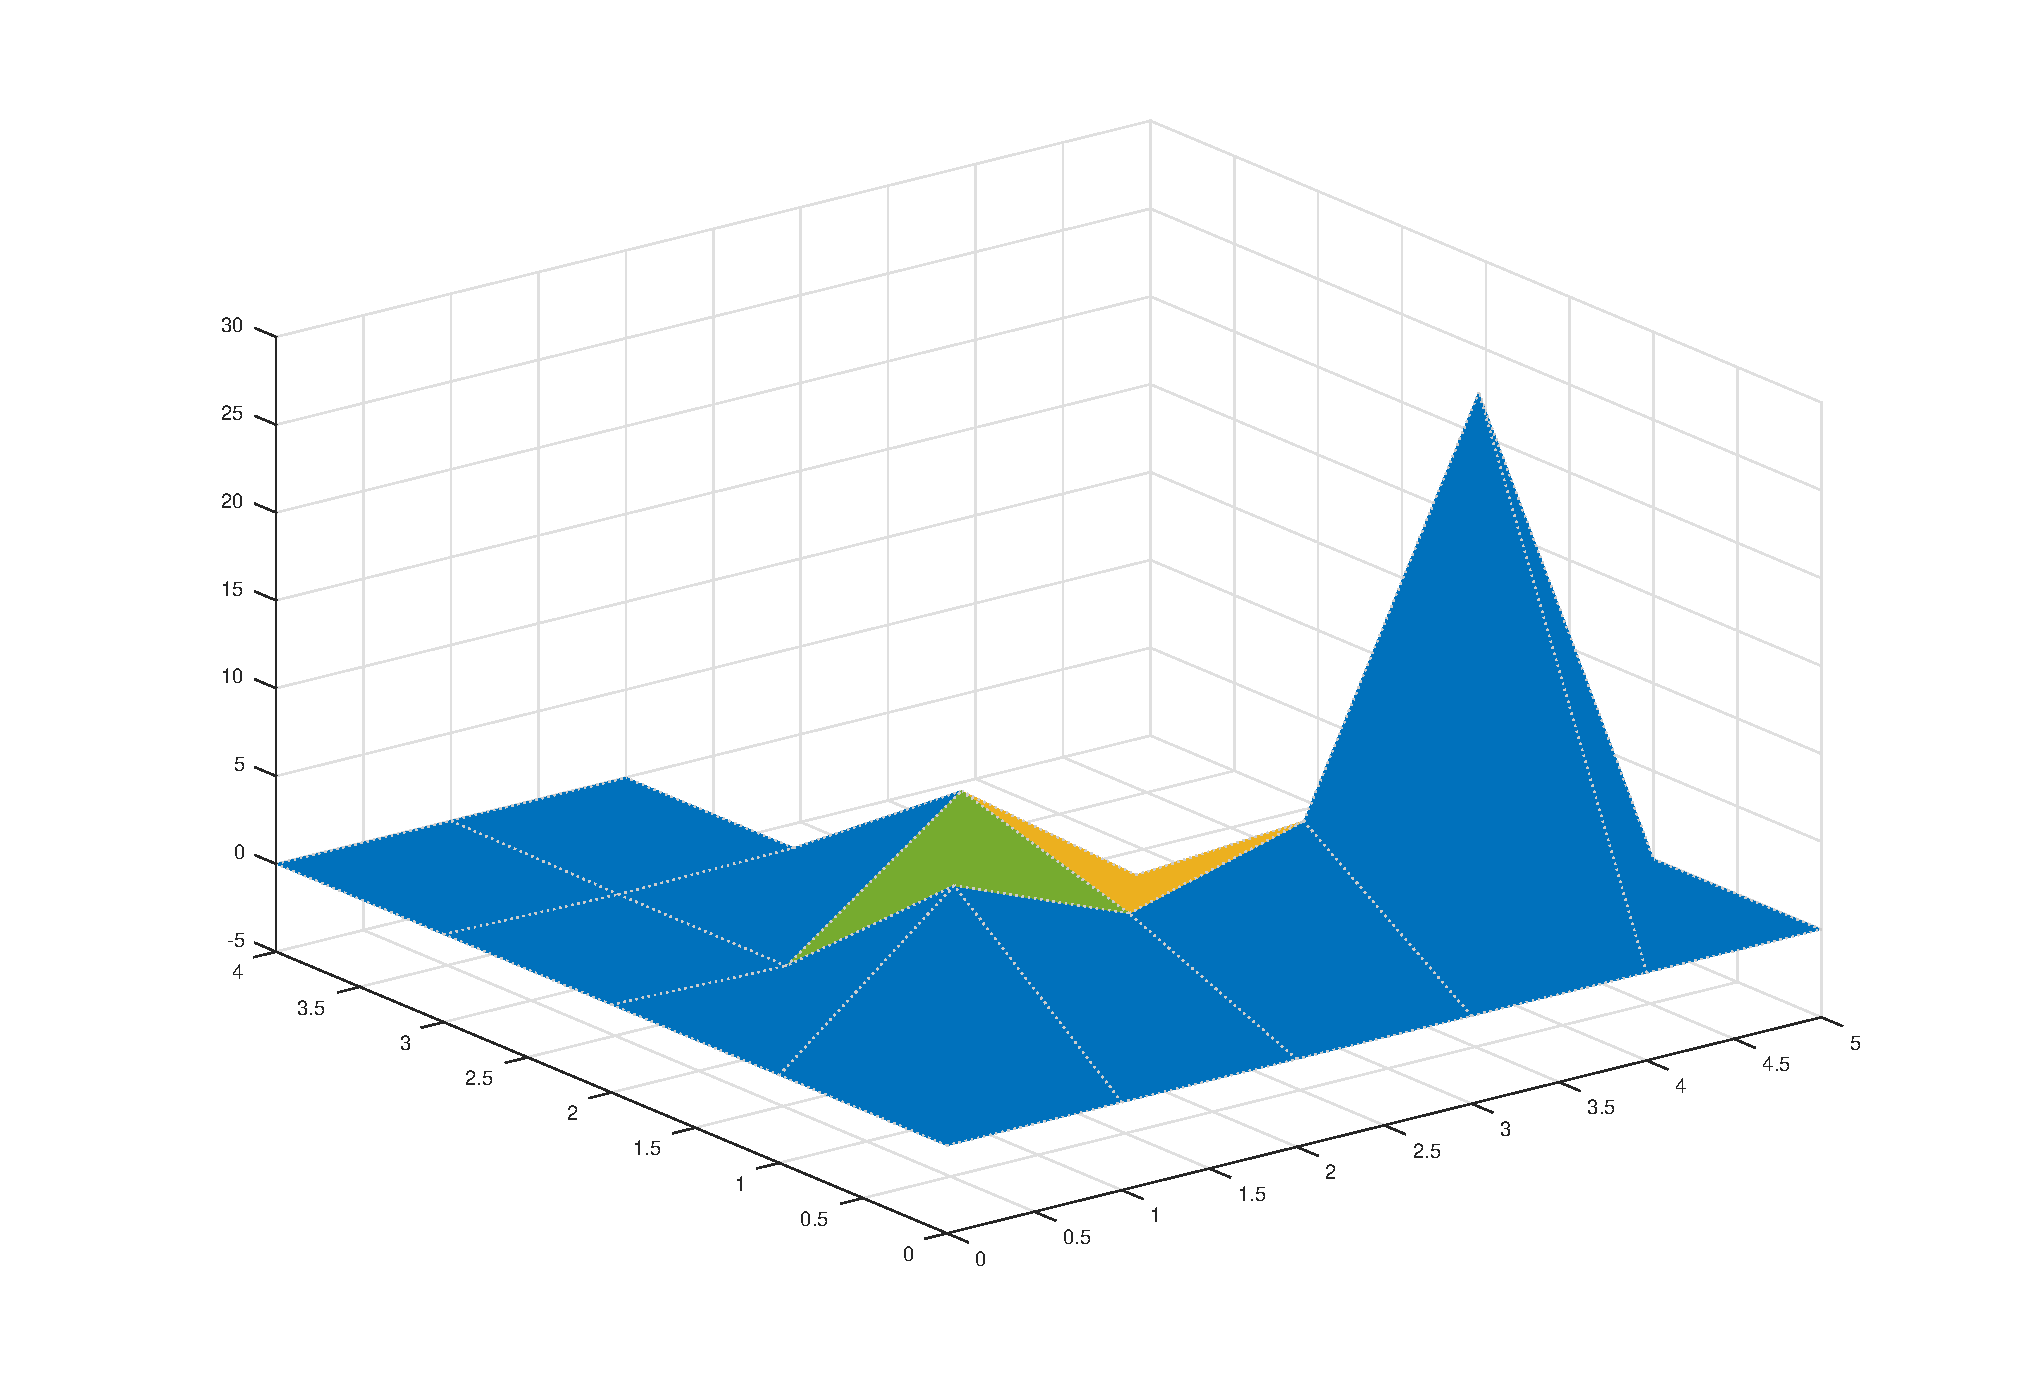
\includegraphics[width=0.5\textwidth]{figures/explicit-h1.eps}
	 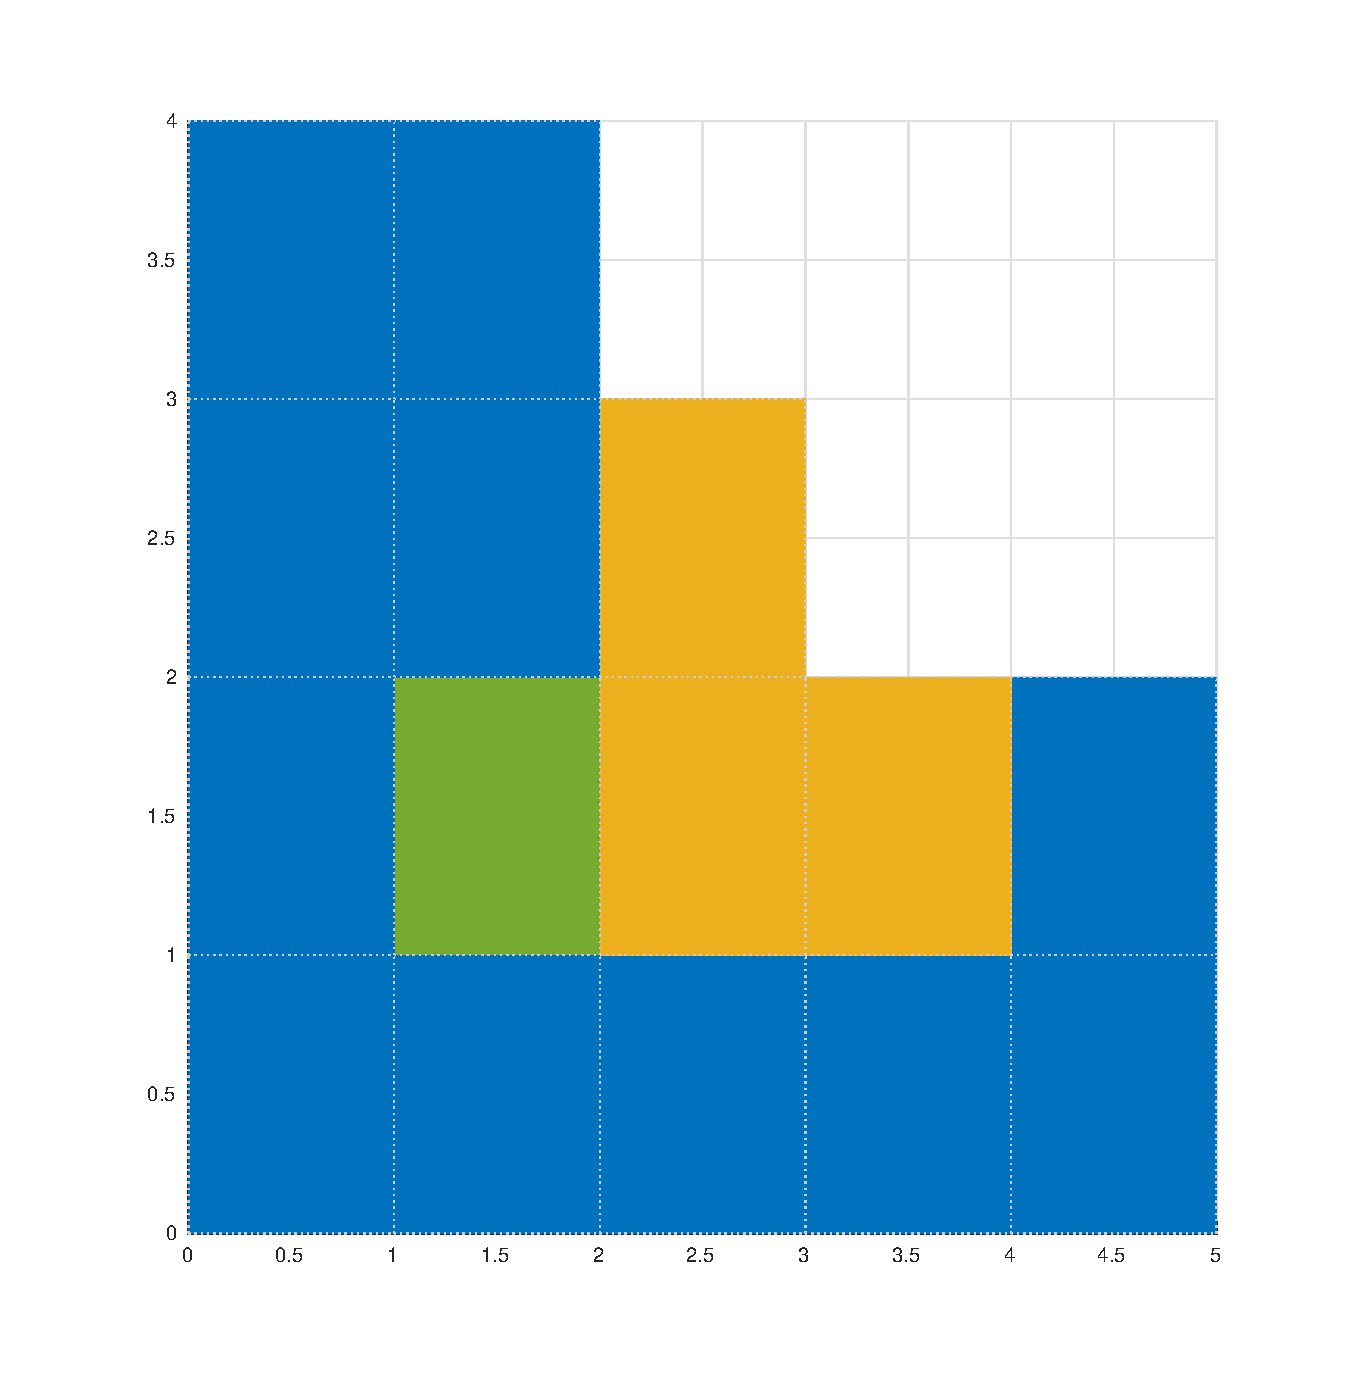
\includegraphics[width=0.5\textwidth]{figures/explicit-h1-top.eps}
	 \caption{Solution with $h=1$}
	 \label{fig: explicit1plot}
 \end{figure}

 \begin{figure}[H]
	 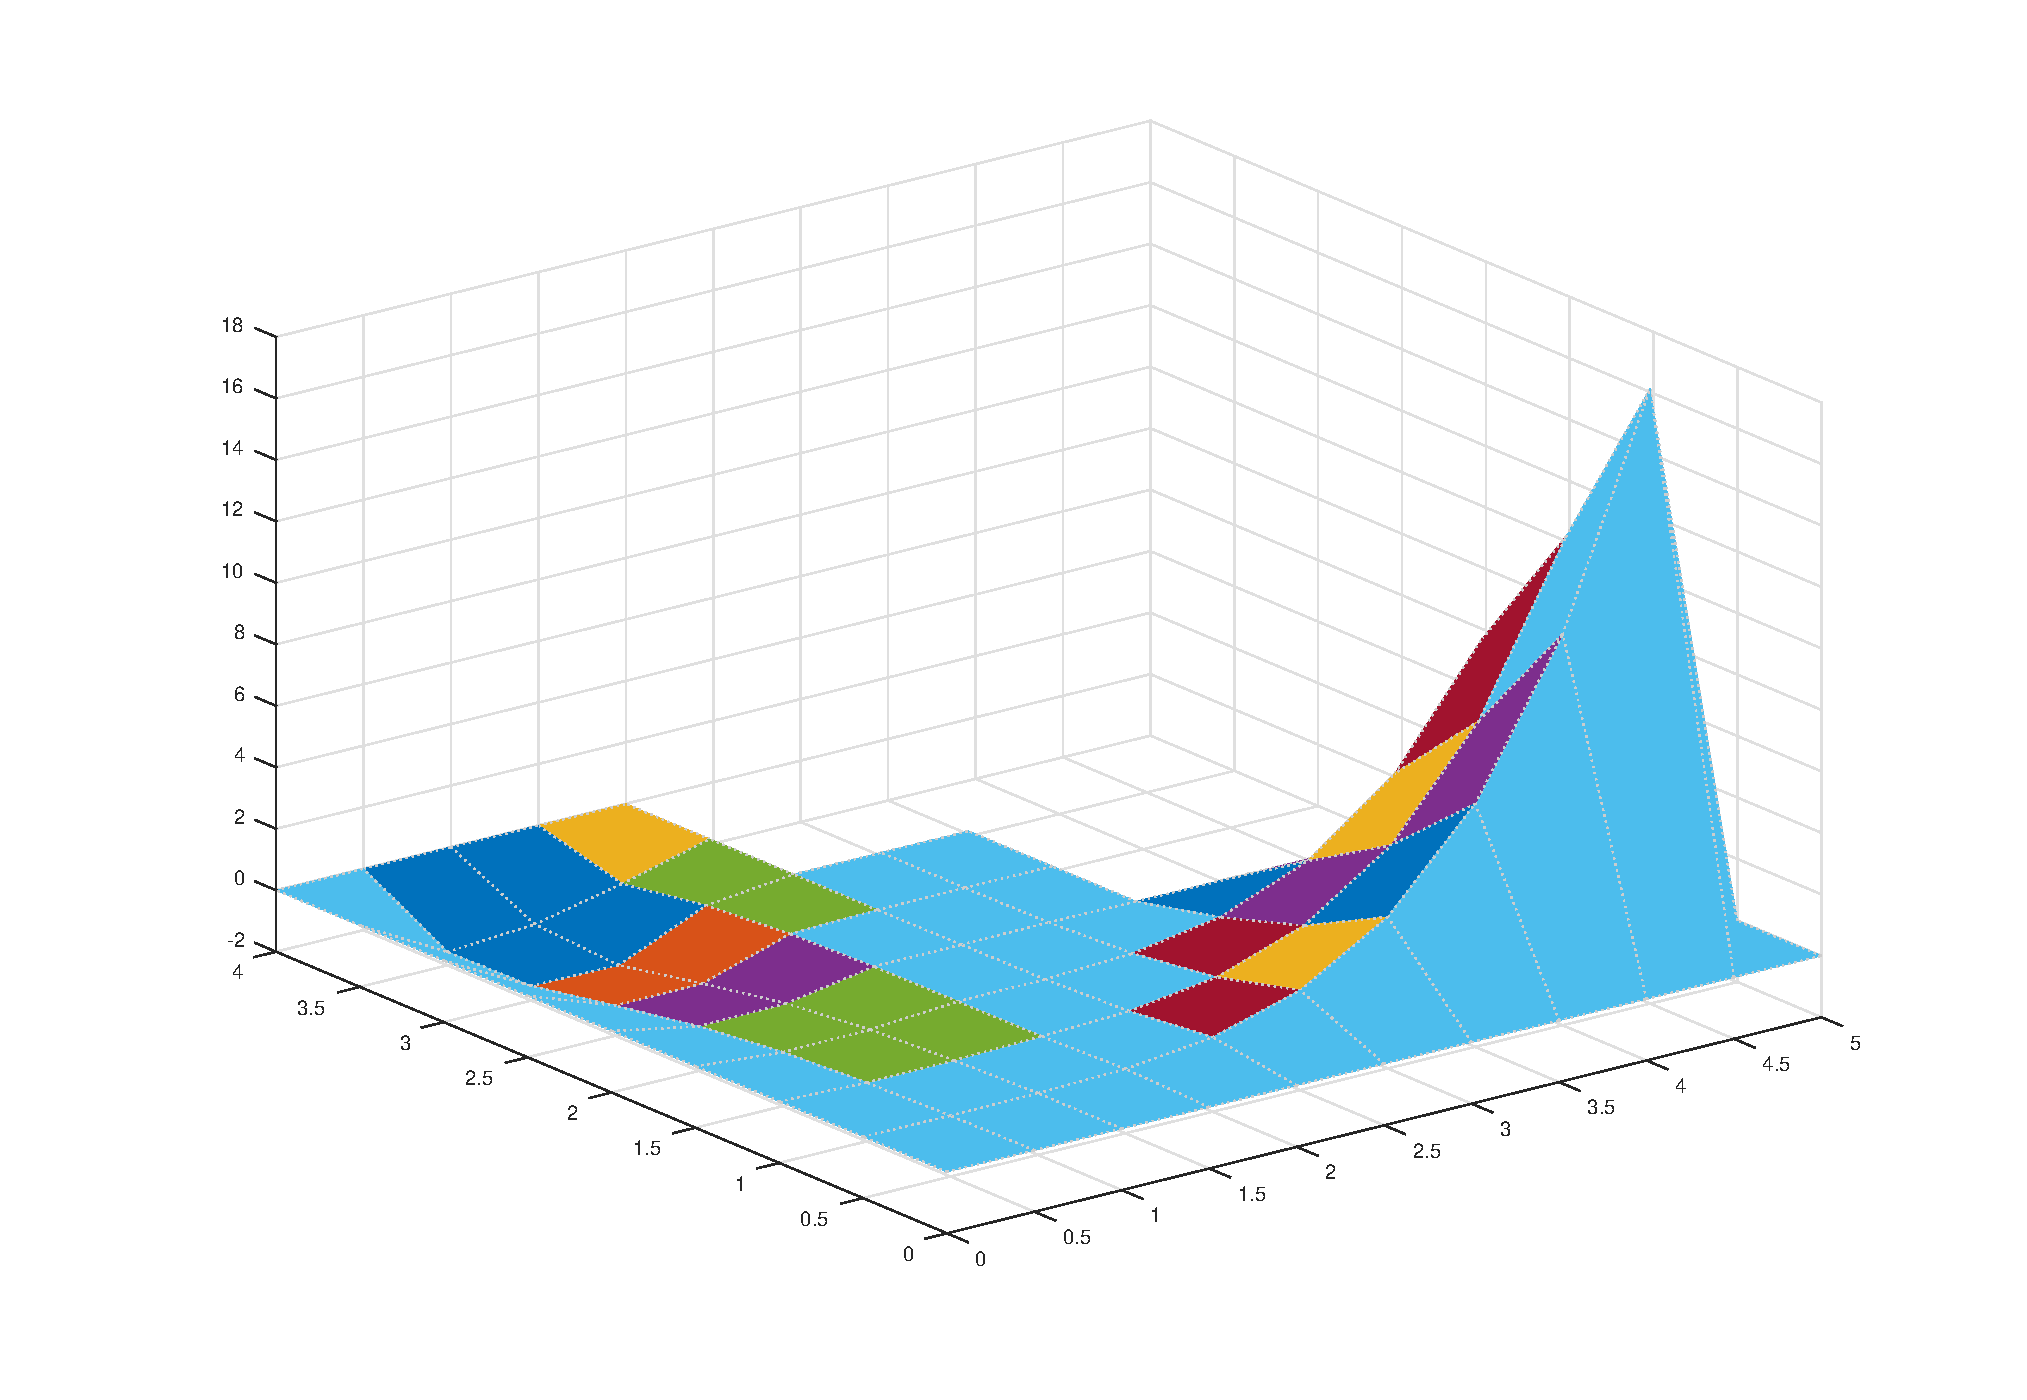
\includegraphics[width=0.5\textwidth]{figures/explicit-h12.eps}
	 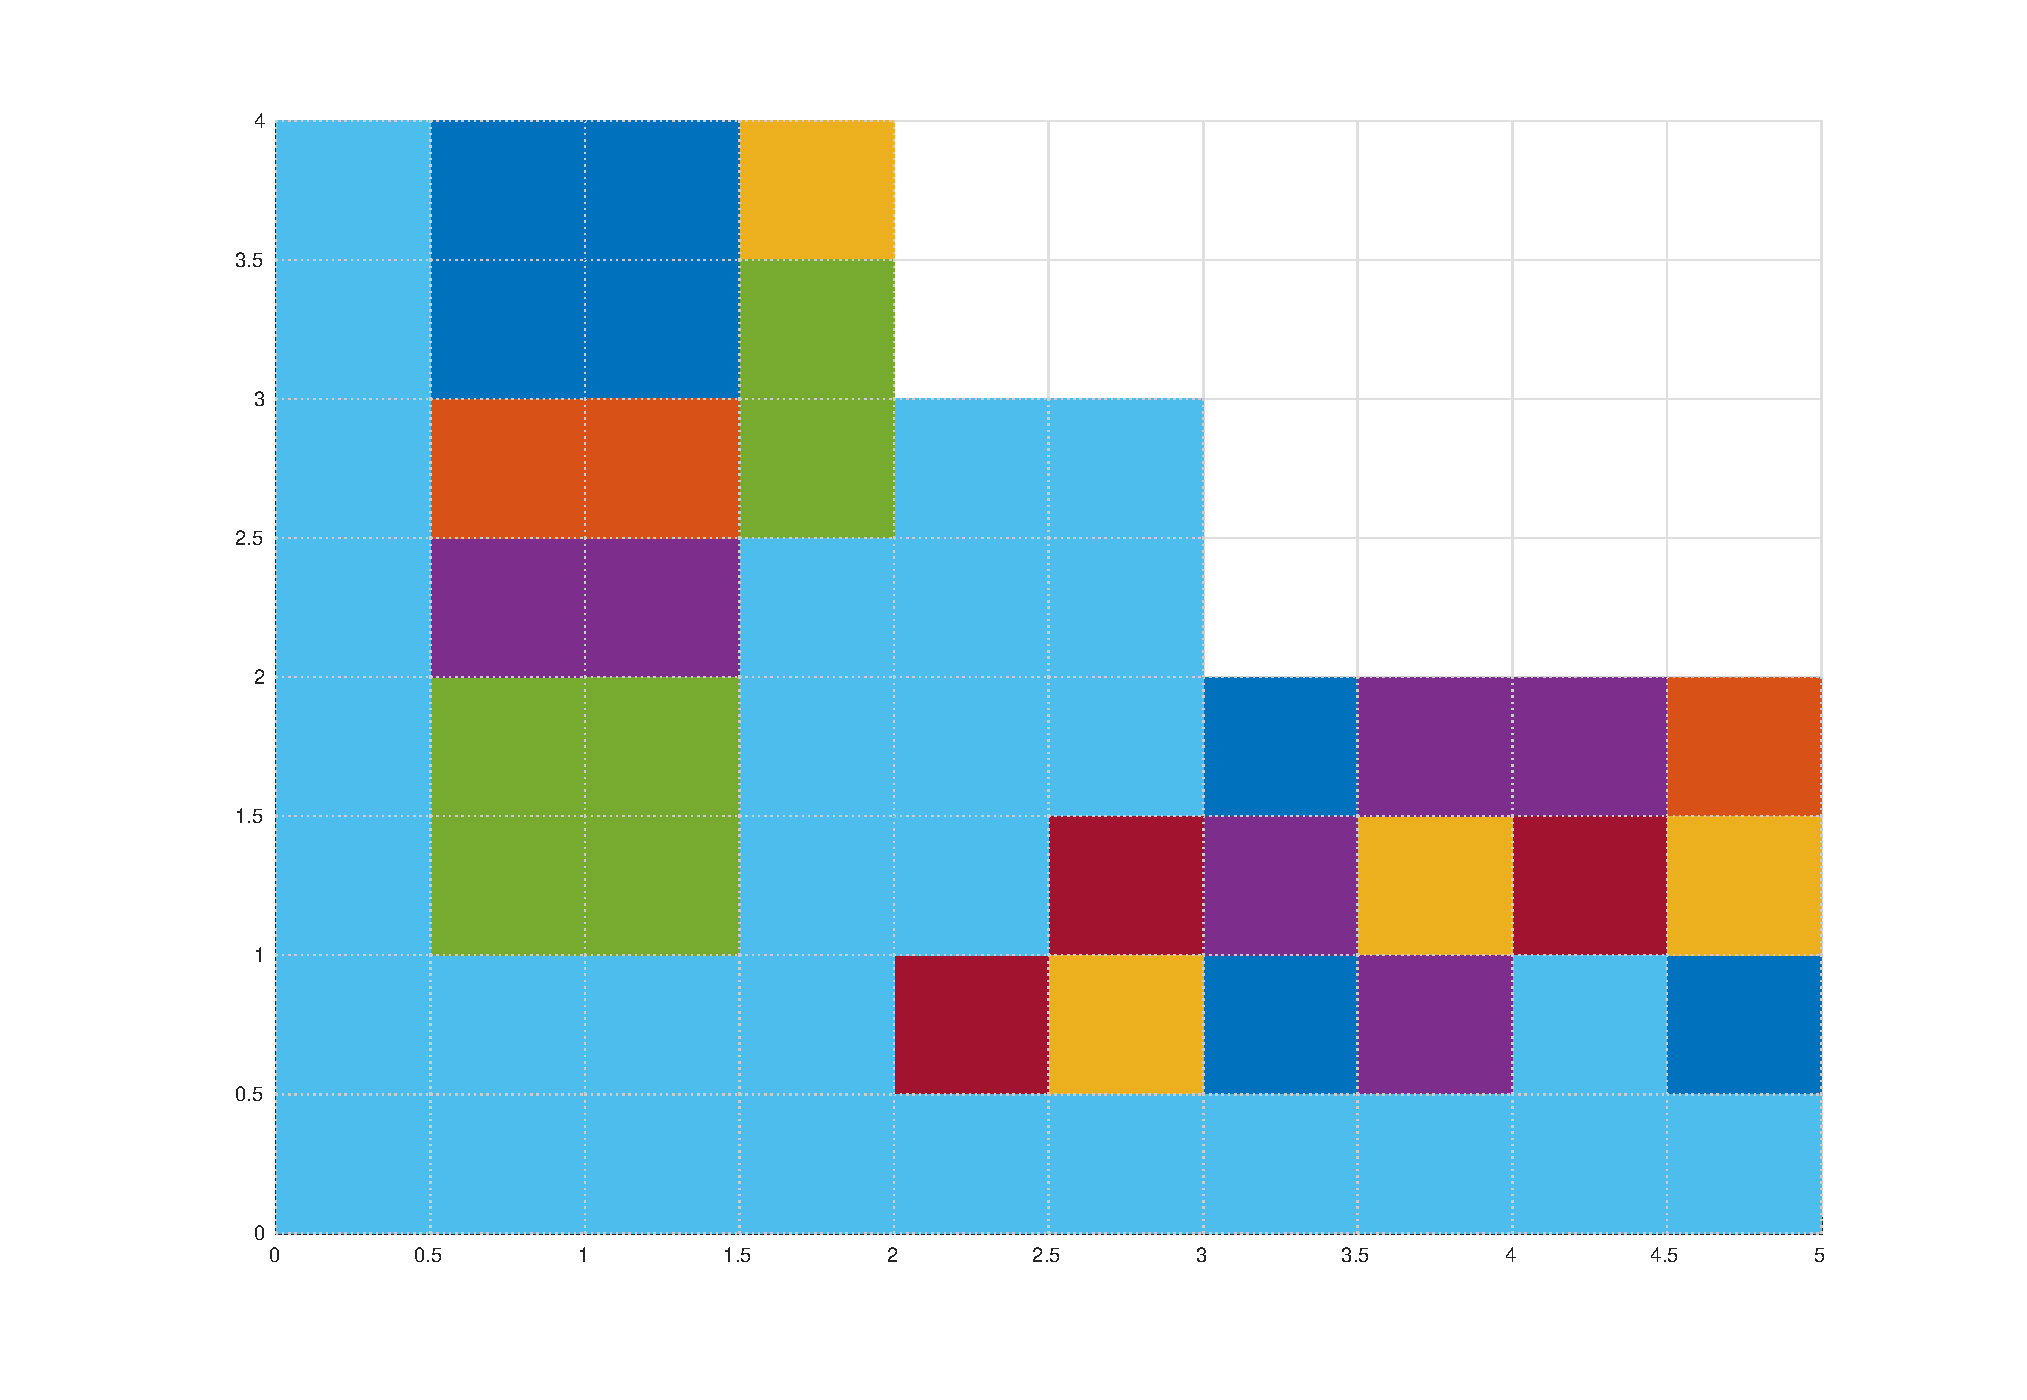
\includegraphics[width=0.5\textwidth]{figures/explicit-h12-top.eps}
	 \caption{Solution with $h=\frac{1}{2}$}
\label{fig: explicit12plot}
 \end{figure}

 \Crefrange{fig: explicit1plot}{fig: explicit12plot} respectively show the solutions with the explicitly solved values of $h$.

\section*{Computational Details}
To solve this problem numerically, MATLAB code was used. Relevant code is shown and the entire function used is attached in listing \ref{lst: centralDifferencePoisson}.

The first step to solving this problem numerically is to create the domain and split it into a mesh based on a step size, which is $\Delta h$ in \cref{eqn: laplacian algebra}. In the code, this was done by using a matrix to represent the points inside the domain. For example, the matrix that represents the domain of interest shown in \cref{fig: domain} is given by

\begin{displaymath}
\left[
\begin{matrix}
1 & 0 & 0 & 0 \\
1 & 1 & 0 & 0 \\
1 & 1 & 1 & 1 
\end{matrix}
\right]
\end{displaymath}

As can be seen, the matrix is in $\mathbb{R}^{m \times n}$ where $m$ is the maximum $y$ value of the domain and $n$ is the maximum $x$ value of the domain if the domain is split into unit squares. Within the matrix, a $1$ represents a unit square while a $0$ represents a place that is not in the domain. Using this method, it is easy to use an arbitrary domain. The matrix can be of any dimension and the size can be scaled to more accurately represent features such as curves. This way of representing the domain can even deal with domains with features such as holes.

When the domain is split up into smaller pieces, the unit squares of the domain simply repeat $\frac{1}{\Delta h}$ times in both their column and the next row. For example, when a step size of $\Delta h = \frac{1}{2}$ is used, the above matrix undergoes the transformation

\begin{displaymath}
\left[
\begin{matrix}
1 & 0 & 0 & 0 \\
1 & 1 & 0 & 0 \\
1 & 1 & 1 & 1 
\end{matrix}
\right]
\to
\left[
\begin{matrix}
	1 & 1 & 1 & 0 & 0 & 0 & 0 & 0 & 0\\
	1 & 1 & 1 & 0 & 0 & 0 & 0 & 0 & 0\\
	1 & 1 & 1 & 1 & 1 & 0 & 0 & 0 & 0\\
	1 & 1 & 1 & 1 & 1 & 0 & 0 & 0 & 0\\
	1 & 1 & 1 & 1 & 1 & 1 & 1 & 1 & 1\\
	1 & 1 & 1 & 1 & 1 & 1 & 1 & 1 & 1\\
	1 & 1 & 1 & 1 & 1 & 1 & 1 & 1 & 1
\end{matrix}
\right]
\end{displaymath}

For this reason, we must choose $\Delta h \leq 1$, although it is already known that a smaller $\Delta h$ yields better results. This expansion of matrices is handled by using a kronecker product to expand the rows and columns by the step size followed by adding a row and column for the missing points, as the first expanded row and column will have an extra for each step.
\pagebreak
\lstinputlisting[language=Matlab, firstline=9, lastline=22, firstnumber=9]{centralDifferencePoisson.m}

This section of the code is very fast, even on quite large matrices. It would likely have greater performance if the \lstinline[language=Matlab]|for| loops were changed to \lstinline[language=Matlab]|parfor| loops, although memory and performance limitations cause issues with solving \cref{eqn: linear system 2} much more quickly than the formation of the matrices in the above code.

The next step is to create the operator matrix $\tilde{\hat{A}}$. Due to the $4u_{ij}$ term in \cref{eqn: laplacian algebra}, it is known that the diagonals of $\tilde{\hat{A}}$ are 4, so an identity matrix is created and multiplied by $4$. The interacting points are found by finding points in the expanded domain with MATLAB's \lstinline[language=Matlab]|find| function and inspecting the points above, below, left, and right, of the current point. This is the slowest portion of the code other than solving the system. As with the expansion of the domain, the performance of this code could be increased by using more parallel code, but solving the system is a much more pressing performance issue.

\lstinputlisting[language=Matlab, firstline=24, lastline=53, firstnumber=24]{centralDifferencePoisson.m}


The interior structure of the matrix can be seen using MATLAB's spy command and is found to be what is shown in \cref{fig: operator matrix}. From this, it is clear that the matrix is sparse; that is, most of its elements are 0. This allows an optimization in MATLAB by using a sparse matrix. Using a sparse matrix to represent the operator matrix  for a step size of $h = \frac{1}{128}$ reduced memory usage from $~450$GB to $~400$MB -- roughly a difference of three orders of magnitude! This allows nearly any machine to compute solutions for small step sizes, although processing time can be significant.

\begin{figure}[H]
\center
\includegraphics[scale=0.3]{figures/operator-spy.eps}
\caption{Operator Matrix Structure}
\label{fig: operator matrix}
\end{figure}

The final step before solving the linear system with MATLAB's built-in functions is to form the right-hand side of \cref{eqn: linear system 2}. This is simply done by evaluating $f(x,y)$ at each of the  points in the domain and put the results in an array and multiply that array by $\left( \Delta h \right)^2$. This is done in the code by a vector operation

\lstinputlisting[language=Matlab, firstline=55, lastline=56, firstnumber=55]{centralDifferencePoisson.m}

Now, the linear system is ready to be solved using built-in functions.

\lstinputlisting[language=Matlab, firstline=58, lastline=73, firstnumber=55]{centralDifferencePoisson.m}

In addition to solving the system,  the code snippet above finds points that are out of the domain and removes them from the variables for the $x$ and $y$ points so the domain is plotted properly.

\section*{Conclusion}

The code presented in this report was used to solve the Poisson equation with the right hand sides

\begin{subequations}
\begin{align}
f(x, y) =& x e^{-x^2 - y^2} \label{eqn: gaussian}\\
f(x, y) =& x \left( x - y \right)^3 \label{eqn: cubic}
\end{align}
\end{subequations}

with $\Delta h = \frac{1}{64}$. The solution plots were then compared with the solutions found by MATLAB's PDE toolbox. These plots are shown in \crefrange{fig: gaussian solutions}{fig: pdetool cubic solutions} on the following pages. The plots in \cref{fig: steps} show the effect of step sizes of $1, 2, 4, 8$ and the rapid approach to the expected solution.



Overall, this method generates very good results with the differential equation and boundary in this case. Due to the flexible nature of how the domain was implemented, it is expected that this method would work for many other domains. Compared to MATLAB's PDE toolbox, the results are slightly worse although the code is likely much simpler. This method takes a similar amount of time to MATLAB's PDE toolbox to run, which is a good sign. The performance could likely be improved by creating more parallel code and carefully profiling the code.

An additional approvement could be made in the representation of the domain. Although the matrix representation of domain points works very well and allows for features such as holes in the domain, it is not easily tested and new bugs may be found when a different domain is used. An improvement to this would be a more advanced system of using a graph data structure to represent the domain. In this system, the nodes would represent points in space. These points could be inside or outside of the domain or be on the boundary of the domain. The edges in the graph would be used to split points to subdivide the points. This would allow the domain to no longer be restricted to rectangles or two dimensions; however, this increase in generality would also require the derivation of a more general operator matrix.


\pagebreak
\subsection*{Solution Plots}

\begin{figure}[H]
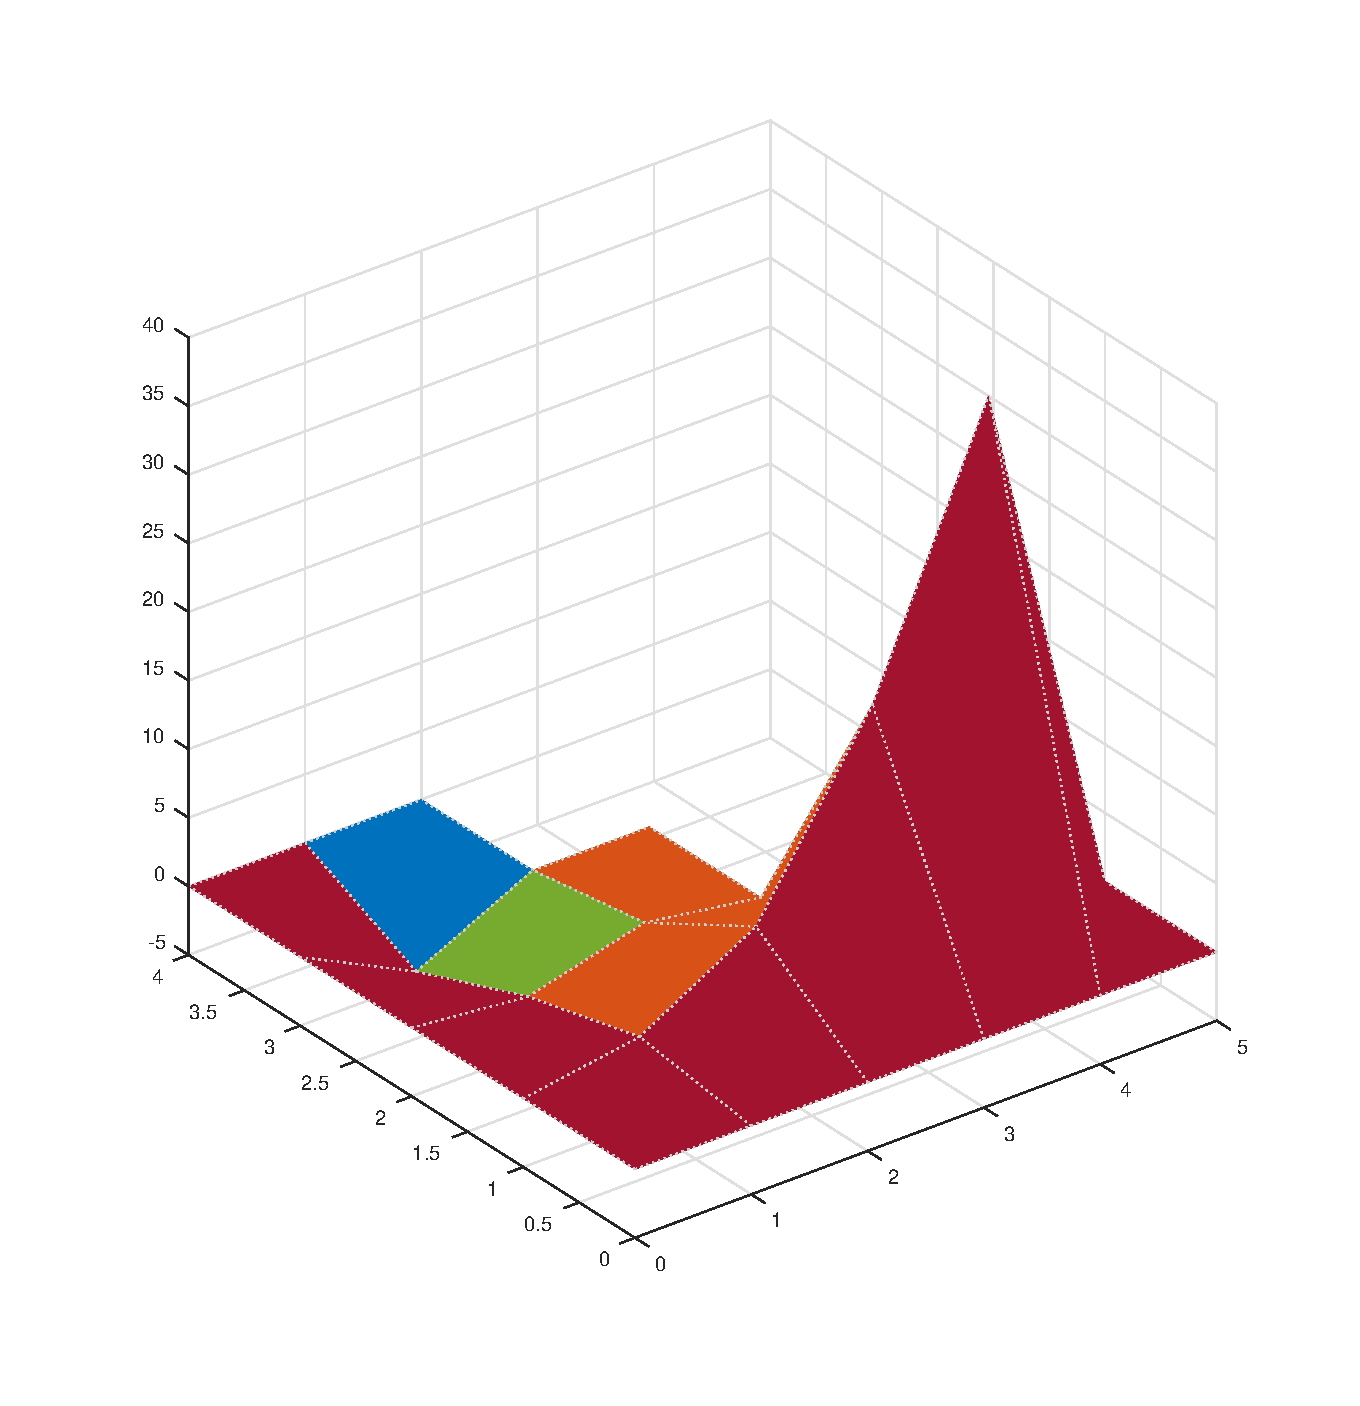
\includegraphics[width=0.5\linewidth]{figures/cubic-1.eps}
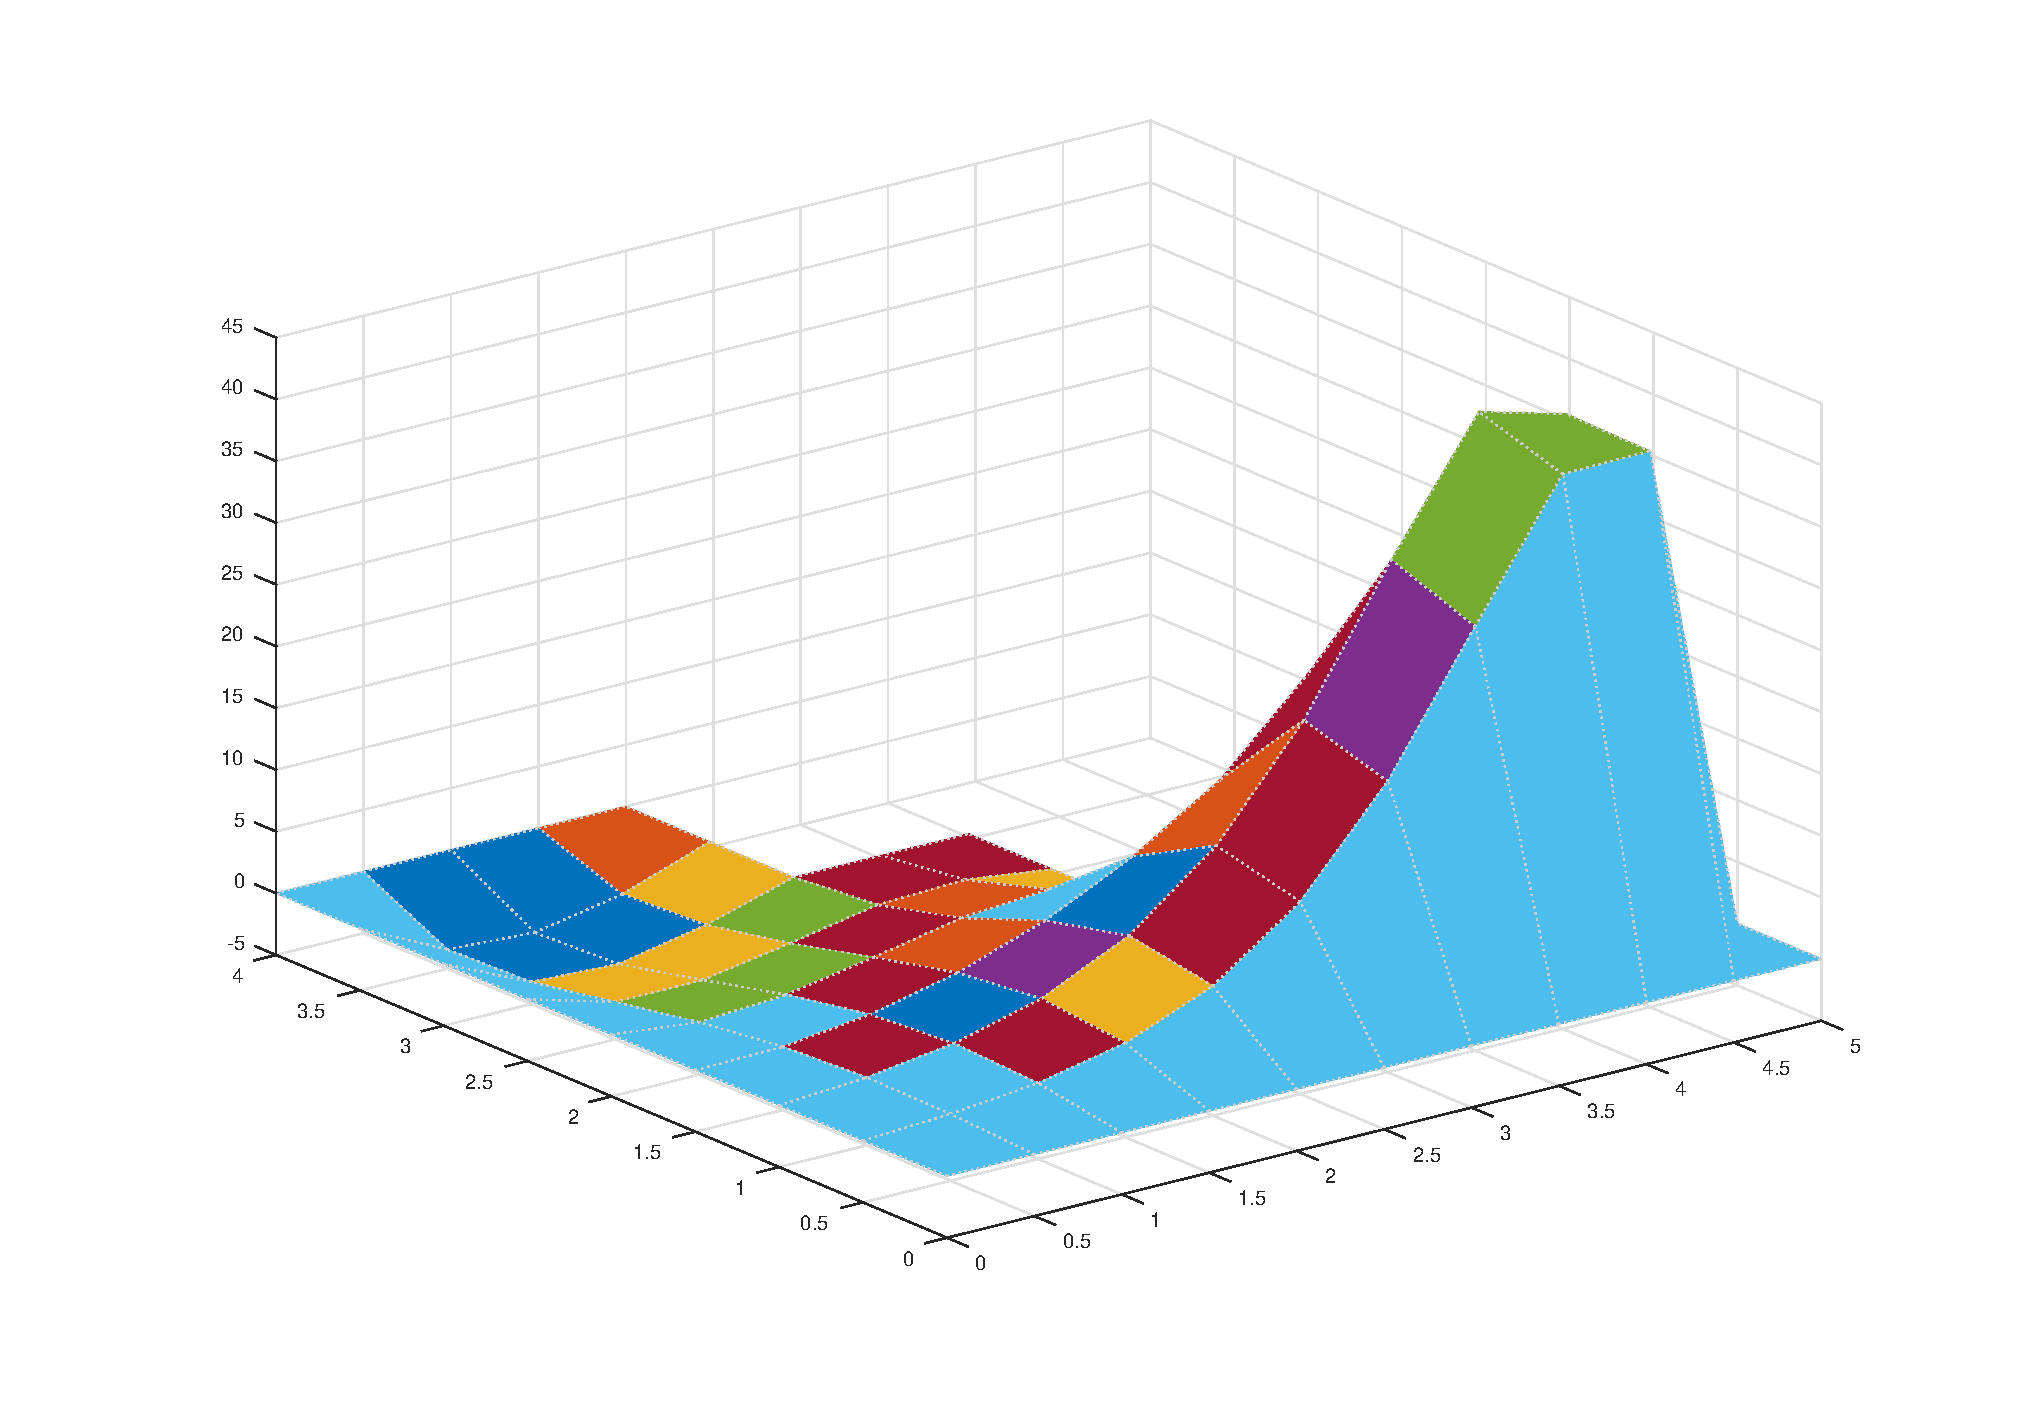
\includegraphics[width=0.5\linewidth]{figures/cubic-2.eps}
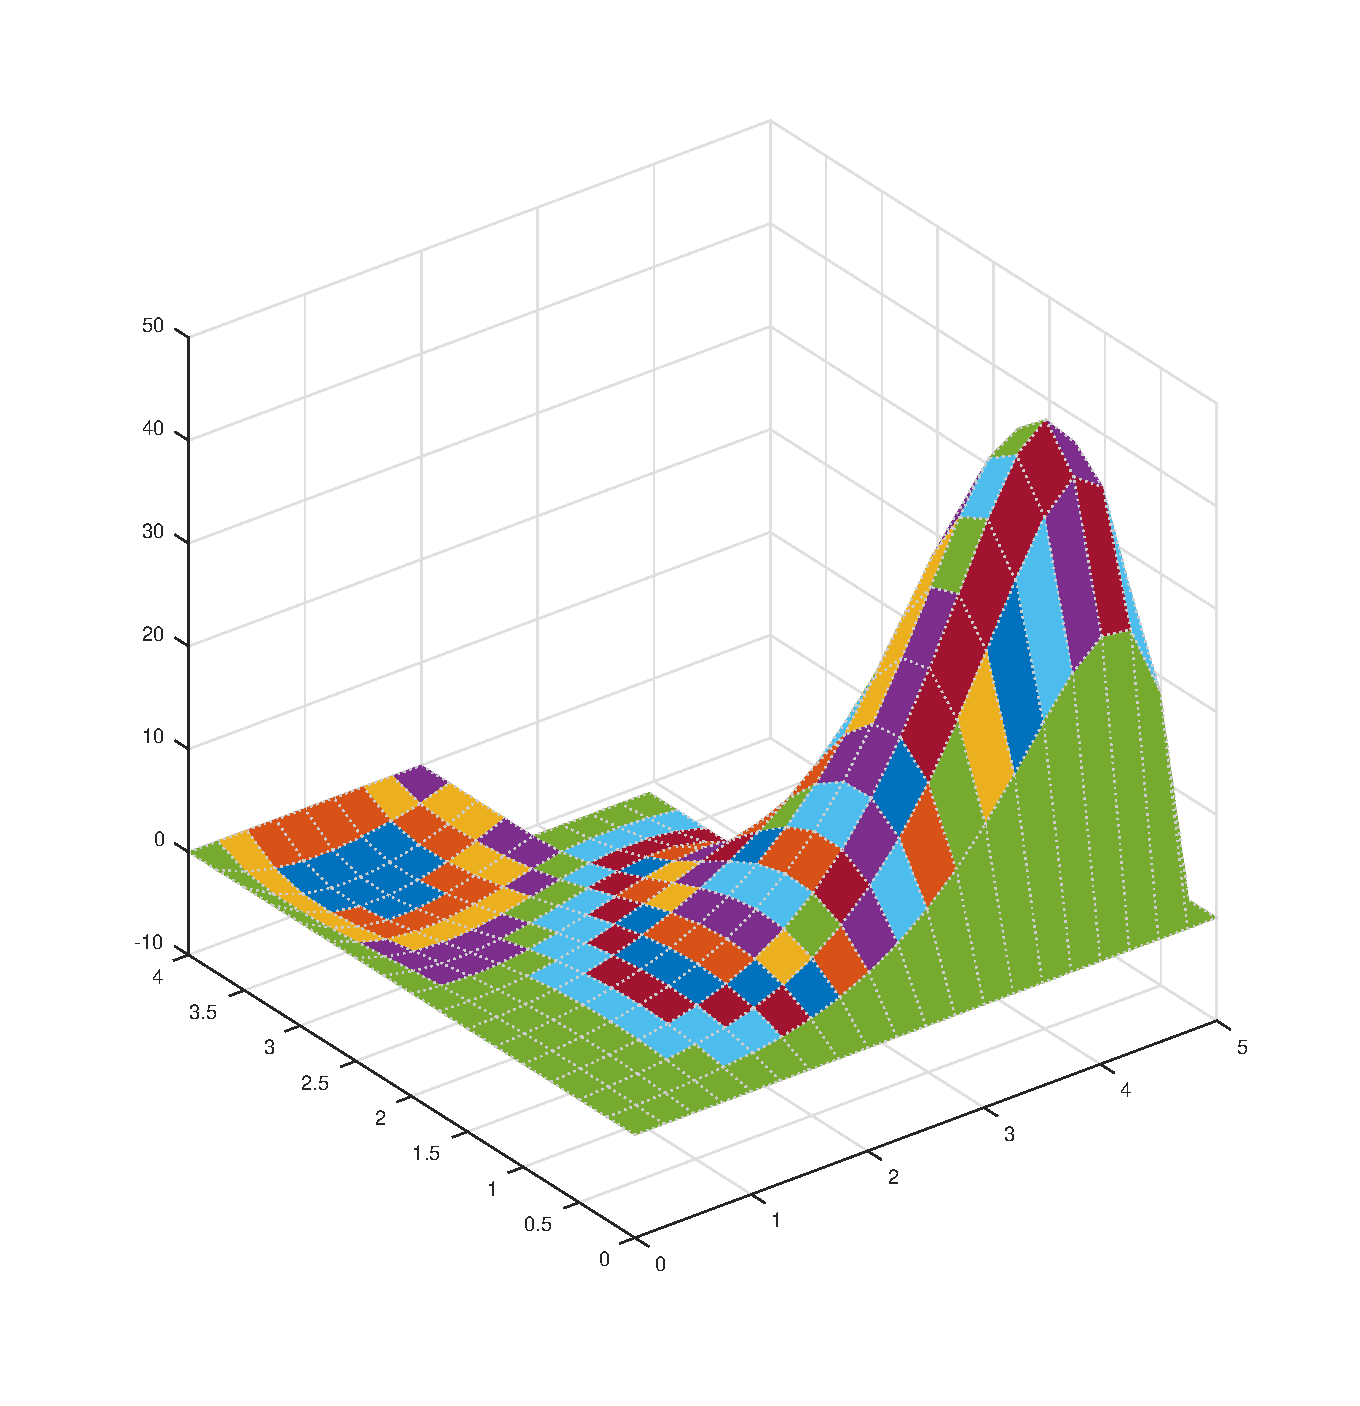
\includegraphics[width=0.5\linewidth]{figures/cubic-4.eps}
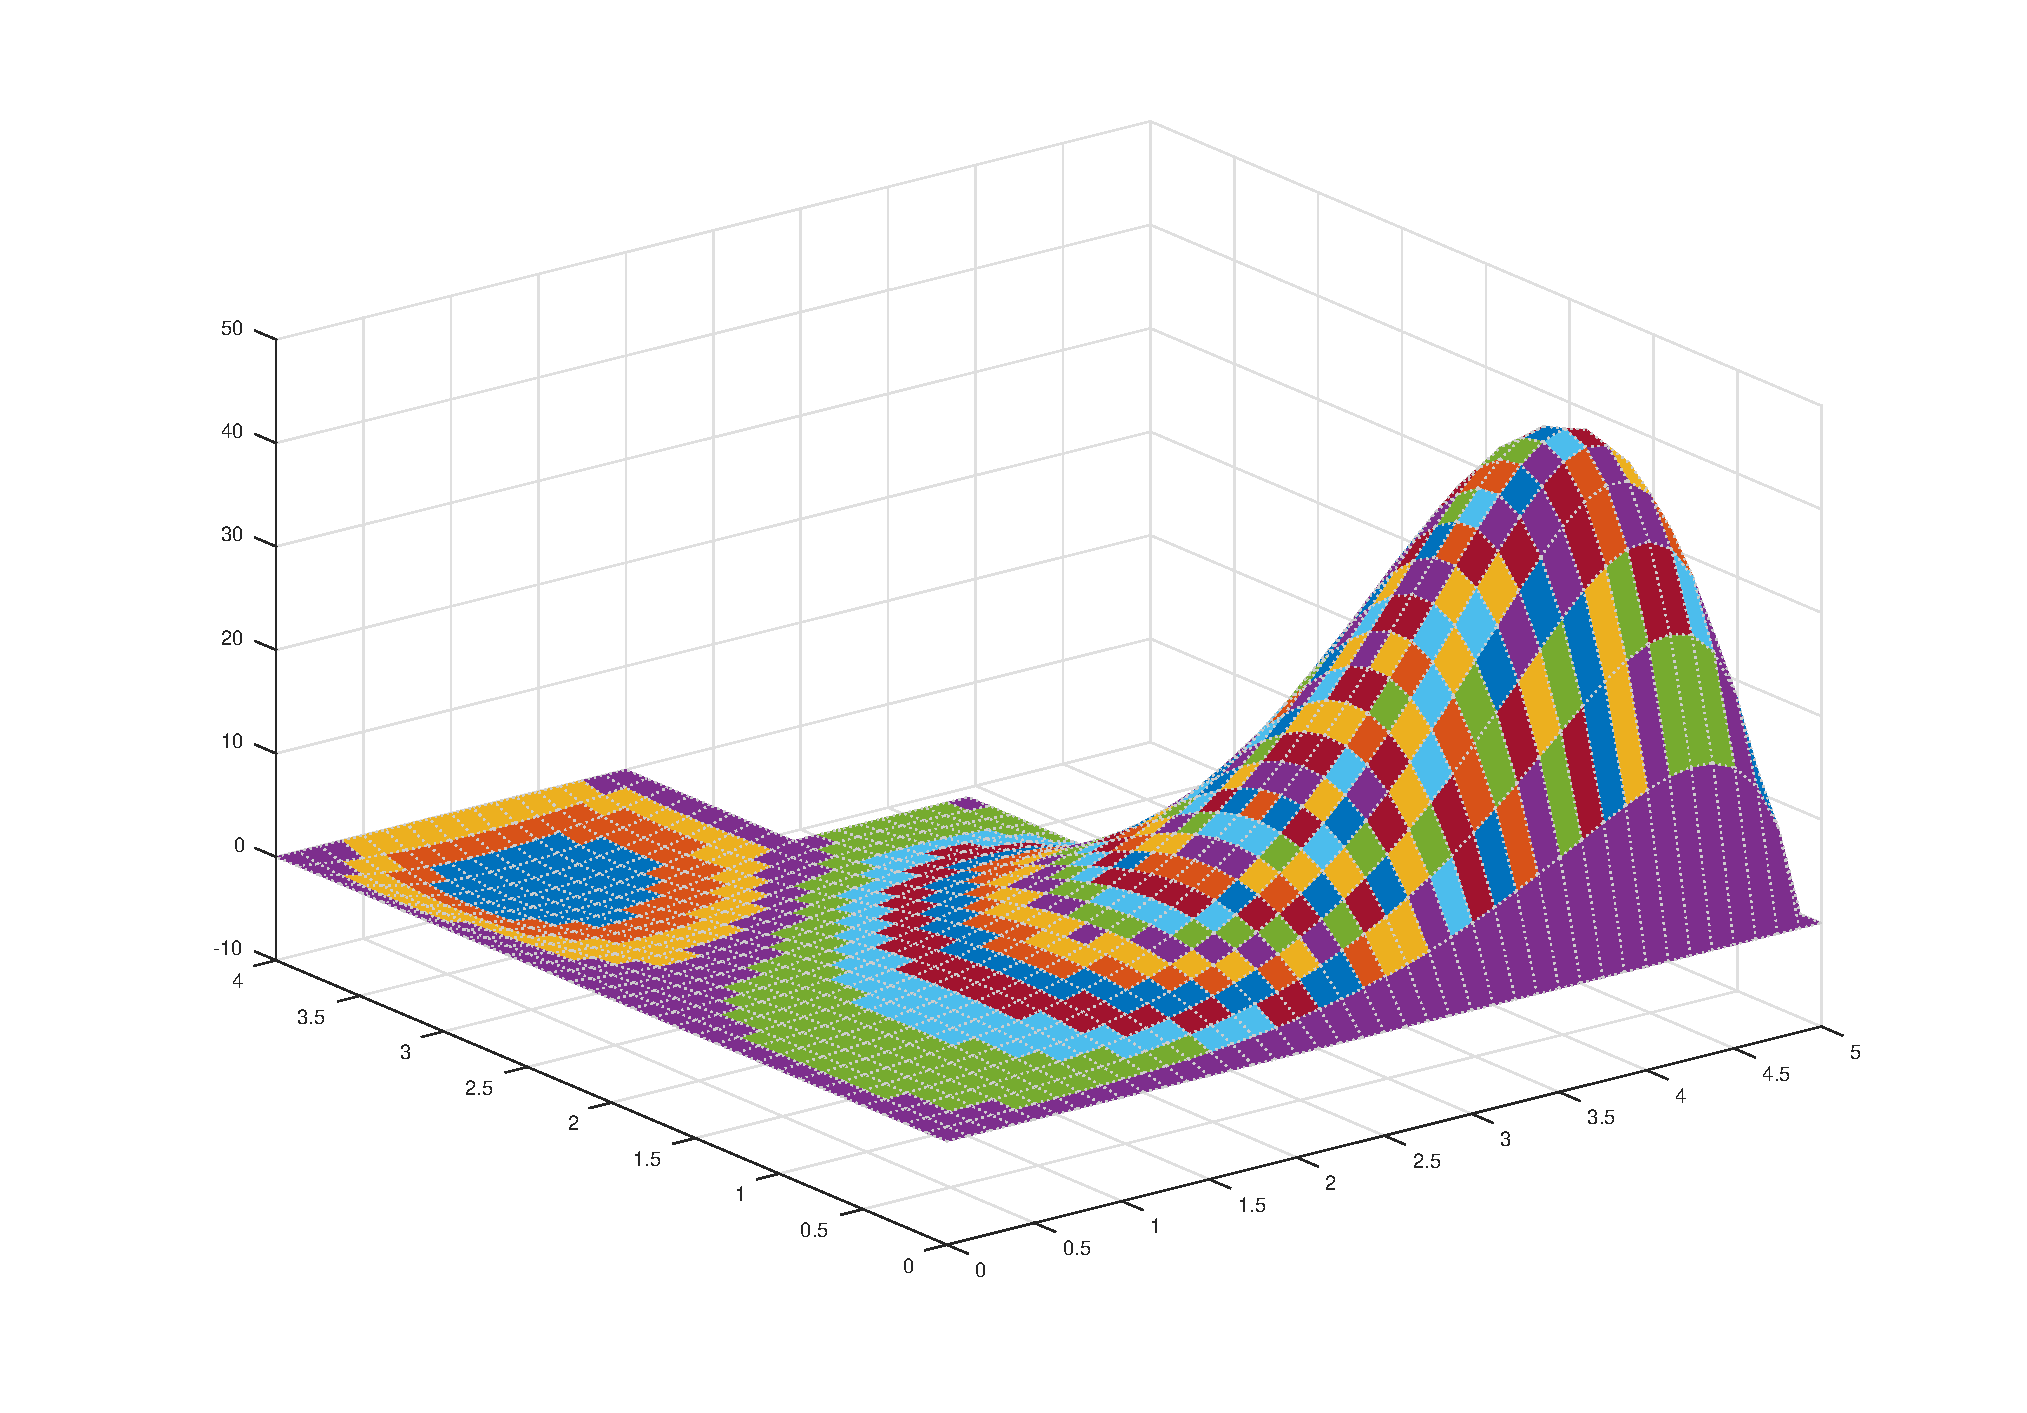
\includegraphics[width=0.5\linewidth]{figures/cubic-8.eps}
\caption{Solutions to \Cref{eqn: cubic} with $\Delta h = 1, 2, 4, 8$}
\label{fig: steps}
\end{figure}

\begin{figure}[H]
\includegraphics[width=\linewidth]{figures/gaussian-64-top.eps}
\includegraphics[width=\linewidth]{figures/gaussian-64.eps}
\caption{Solutions to \Cref{eqn: gaussian}}
\label{fig: gaussian solutions}
\end{figure}

\begin{figure}[H]
\includegraphics[width=\linewidth]{figures/gaussian-top-pdetool.png}
\includegraphics[width=\linewidth]{figures/gaussian-iso-pdetool.png}
\caption{PDE Toolbox Solutions to \Cref{eqn: gaussian}}
\label{fig: pdetool gaussian solutions}
\end{figure}

\begin{figure}[H]
\includegraphics[width=\linewidth]{figures/cubic-64-top.eps}
\includegraphics[width=\linewidth]{figures/cubic-64.eps}
\caption{Solutions to \Cref{eqn: cubic}}
\label{fig: cubic solutions}
\end{figure}

\begin{figure}[H]
\includegraphics[width=\linewidth]{figures/cubic-top-pdetool.png}
\includegraphics[width=\linewidth]{figures/cubic-iso-pdetool.png}
\caption{PDE Toolbox Solutions to \Cref{eqn: cubic}}
\label{fig: pdetool cubic solutions}
\end{figure}

\newpage
\section*{Full Code Listing}

Below is a listing of the code used for this report. The most recent code is available in the source repository at \url{https://github.com/danielunderwood/poisson-central-difference} and the most recent compiled version of the report is available at \url{https://www.sharelatex.com/github/repos/danielunderwood/poisson-central-difference/builds/latest/output.pdf}.

\lstinputlisting[language=Matlab, caption=explicit\_h1\_solver.m, label={lst: explicit1}]{explicit_h1_solver.m}
\lstinputlisting[language=Matlab, caption=explicit\_h12\_solver.m, label={lst: explicit12}]{explicit_h12_solver.m}
\lstinputlisting[language=Matlab, caption=centralDifferencePoisson.m, label={lst: centralDifferencePoisson}]{centralDifferencePoisson.m}


\end{document}
